\documentclass[12pt]{article}

\usepackage{fontawesome}
\usepackage{hyperref}
\usepackage{xurl}
\usepackage{graphicx}
\usepackage{float}
\usepackage[tagged, highstructure]{accessibility}
\usepackage{bookmark}
\usepackage{enumitem}

\hypersetup{
    colorlinks=false,
    pdfborder={0 0 0},
    pdftitle={SQL Review},
    pdfauthor={Adrianna Holden-Gouveia},
    pdfsubject={Advanced Data - Lab Assignment},
    pdflang={en-US},
    pdfkeywords={SQL, queries, database, SQL Bolt, review}
}

% Configure PDF bookmarks for navigation
\bookmarksetup{
    numbered,
    open,
}

% Configure list spacing for better accessibility
\setlist{nosep}



\title{SQL Review}
\author{
        Adrianna Holden-Gouveia \\
        Website: \href{https://aholdengouveia.name}{aholdengouveia.name}\\ 
        \date{\vspace{-5ex}}
        %Email: \href{mailto:admin@aholdengouveia.name}{admin@aholdengouveia.name} \\
%        \faLinkedin{: aholdengouveia} \\
        \faGithub {: aholdengouveia} \\
        %\faTwitter {: aholdengouveia} \\
        }

%S\date{\today}


\begin{document}    

\maketitle

%\begin{abstract}
%This is a template for Linux Administration Lab work
%\end{abstract}
%\tableofcontents


\section*{Accessibility Notice}
This document is also available in HTML format at:

Link: \href{https://aholdengouveia.name/AdvData/labs/week2.html}{\textbf{\nolinkurl{https://aholdengouveia.name/AdvData/labs/week2.html}}}

The HTML version provides enhanced accessibility features including keyboard navigation, screen reader support, responsive design, dark mode support, and high contrast options.

\section*{Request}
\noindent\textbf{Request:} DATA-3172\\
\textbf{Requested by:} Operations manager at your company\\
\textbf{Data:} Your data set from the Introduction to Data lab

\section*{Background}
Before anyone relies on this data, your manager wants to see that it can answer real business questions, and that your queries are documented so the rest of the team can reuse them. You'll start with a quick SQL refresher as training, then load your data into a database and put it to work.

\section*{Learning Outcomes}
By the end of this lab, you will be able to:
\begin{itemize}
    \item Write basic SQL queries to select, filter, and sort data
    \item Explain what each part of a SQL query does
    \item Turn business questions about your data set into documented SQL queries, with a business justification for each
    \item Evaluate a SQL tutorial, including where you needed help
\end{itemize}

\section*{Lab Instructions}

\subsection*{Screenshots}
Several parts of this lab ask for a screenshot. Each screenshot should have your name, term, and year.  One of the easiest ways to do that is make a text document with your name and term/year on your computer and save it to use all term. Any screenshots that don't include this information won't be counted.

\begin{figure}[H]
    \centerline{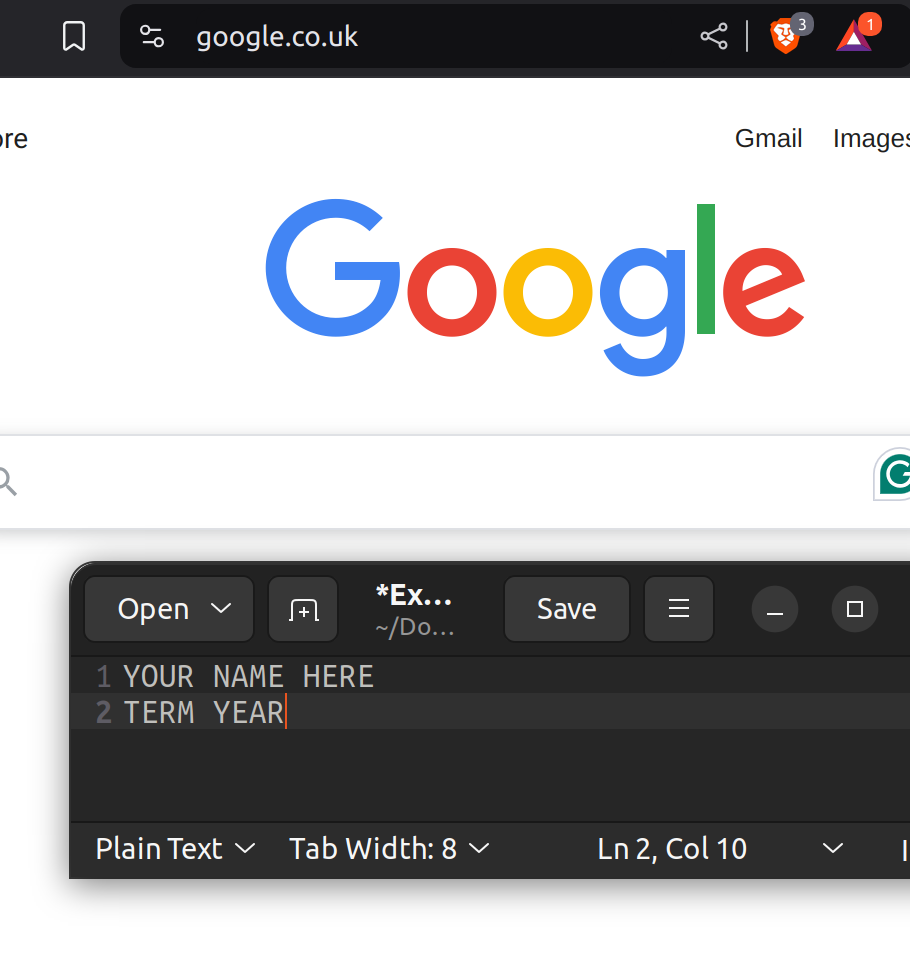
\includegraphics[scale=.2]{ExampleScreenshot.png}}
    \caption{This is an image of what each of your screenshots should look like}
    \alt{Example screenshot: a web browser showing the Google home page, with a small text editor window in front of it that says YOUR NAME HERE and TERM YEAR}
\end{figure}

\subsection*{Part 1: SQL Review Tutorial}
Go through these 5 sections of SQLBolt (linked under Resources), and complete the exercises at the end of each one:
\begin{itemize}
    \item SQL Lesson 1: SELECT queries 101
    \item SQL Lesson 2: Queries with constraints (Pt. 1)
    \item SQL Lesson 3: Queries with constraints (Pt. 2)
    \item SQL Lesson 4: Filtering and sorting Query results
    \item SQL Review: Simple SELECT Queries
\end{itemize}
Take a screenshot of each section after you complete its exercises. Make sure you have the green checkmark on each problem. Then answer these questions:
\begin{enumerate}
    \item Which, if any, questions did you find challenging? Why?
    \item How many of the questions did you need a hint on? Why?
    \item What is your review of this tutorial? What would you change or fix?
    \item Pick one query you wrote and explain what each part does: SELECT, FROM, WHERE, and ORDER BY.
\end{enumerate}

\subsection*{Part 2: Business Questions About Your Data}
Now use SQL on your own data set from the Introduction to Data lab. Books are my example data only, so your questions and queries must be about your own data.
\begin{enumerate}
    \item Load your data set into a database as a single table. You will organize your data into multiple tables later in the term, so one table is fine for now. Here's the way I suggest, which runs in your browser with nothing to install. The tools are linked under Resources.
    \begin{enumerate}
        \item Open my CSV to Database Converter, and choose your CSV file. Keep the first 100 to 1,000 rows, since bigger databases can cause errors in browser tools. Select Convert, check the summary, and download your database.
        \item Open SandboxSQL, use Load a Database, and choose the file you downloaded.
        \item Check that it worked by running SELECT COUNT(*) on your table. The count should match the number of rows the converter showed.
    \end{enumerate}
    You can use a different tool if you prefer, as long as you turn in a database file, not a CSV file or a spreadsheet.
    \item Write 5 business questions that someone at the company from your data card might ask about your data.
    \item Write a query that answers each question. Across your 5 queries, use WHERE, ORDER BY, and at least one WHERE with more than one condition.
    \item Document each query using the format in the sample query documentation (linked under Resources). Each one needs a header comment with the business question, who is asking, a business justification, and any notes, followed by the query and a short summary of the result. Your result summary must quote specific numbers or values from your results, such as how many rows came back or the top value.
    \item Take a screenshot of each query and its results.
    \item Export your database to turn in. In SandboxSQL, use the Export button, which saves it as a .sqlite file. SandboxSQL doesn't always keep your work if you close the page, so export at the end of each session, and use Load a Database to open your .sqlite file next time.
\end{enumerate}

\section*{Acceptance Criteria}
This request is done when:
\begin{itemize}
    \item All 5 SQLBolt sections are complete, with a green checkmark on every problem
    \item Your data is loaded into a database as one table, and your database file is turned in
    \item 5 business questions that someone at your company would actually ask
    \item Each question has a query that runs and returns results that answer it
    \item Each result summary quotes specific numbers or values from your results
    \item Every query is documented in the sample format, with a business justification
    \item Across your queries, you use WHERE, ORDER BY, and at least one WHERE with more than one condition
    \item Every screenshot follows the screenshot rules
\end{itemize}

\section*{Deliverables}
Two files:
\begin{enumerate}
    \item A document that includes Part 1, your 5 SQLBolt screenshots and your answers to the 4 questions, and Part 2, your 5 documented queries with a screenshot of each one and its results
    \item Your database file
\end{enumerate}

Audience: your manager and the rest of the data team.

\section*{Resources}
References, a video, a PowerPoint and some notes are available at my website
Link: \href{https://www.aholdengouveia.name/AdvData/sqlpt1.html}{\textbf{\nolinkurl{https://www.aholdengouveia.name/AdvData/sqlpt1.html}}}

SQLBolt, the tutorial for Part 1
Link: \href{https://sqlbolt.com/}{\textbf{\nolinkurl{https://sqlbolt.com/}}}

Suggested tool: SandboxSQL, free, runs in your browser, and saves your database as a .sqlite file with its Export button
Link: \href{https://www.sandboxsql.com/}{\textbf{\nolinkurl{https://www.sandboxsql.com/}}}

My CSV to Database Converter, which makes a database file from your CSV file
Link: \href{https://www.aholdengouveia.name/AdvData/labs/csv-to-database.html}{\textbf{\nolinkurl{https://www.aholdengouveia.name/AdvData/labs/csv-to-database.html}}}

Optional, if you'd rather install a tool: DB Browser for SQLite, which can import a CSV file directly
Link: \href{https://sqlitebrowser.org/}{\textbf{\nolinkurl{https://sqlitebrowser.org/}}}

Sample query documentation, showing the format to follow
Link: \href{https://www.aholdengouveia.name/AdvData/labs/SampleQueryDocumentation.txt}{\textbf{\nolinkurl{https://www.aholdengouveia.name/AdvData/labs/SampleQueryDocumentation.txt}}}

\end{document}